\section{Algoritma}
\begin{figure}[H]
        \centerline{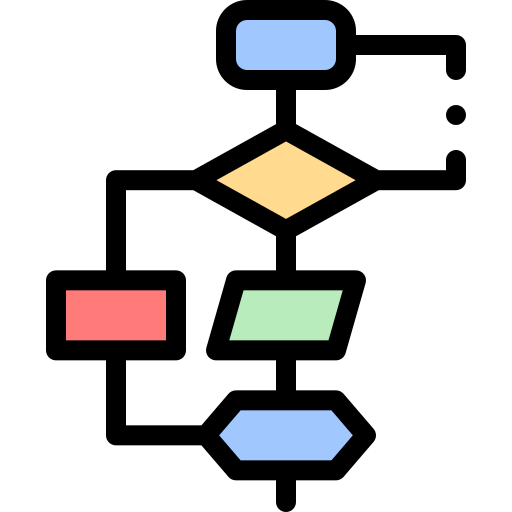
\includegraphics[scale=0.5]{figures/algoritma-kompleksitas/algoritma}}
        \caption{Algoritma}
\end{figure}
sebelum jauh kita bahas tentang yang lainnya, mari kita bahas apa itu Algoritma:

\textit{Algoritma adalah sebuah proses atau seperangkat aturan yang harus diikuti dalam operasi pemecahan masalah}
Sederhananya, algoritma adalah serangkaian proses yang dilakukan secara berurutan untuk menyelesaikan sebuah permasalahan. Algoritma bisa bermacam-macam tergantung kepada siapa yang membuat algoritma tersebut. Namun permasalahannya adalah algoritma mana yang lebih efektif dan efisien? Algoritma sangat banyak digunakan dikehidupan sehari-hari, contohnya adalah bagaimana anda memasak air, bagaimana memasak mie instan, bagaimana menyalakan mesin motor, dan lain sebagainya yang dimana aktivitas tersebut terdapat proses alur yang jika kita ikuti maka akan mencapai suatu tujuan yang ingin kita capai, seperti ingin menyalakan motor contoh yang saya ketahui adalah sebagai berikut,
\begin{enumerate}
\item ambil kunci motor
\item masukkan kunci motor pada \textbf{main switch}
\item putar hingga ke arah on
\item lalu tekan tombol starter pada motor
\item motor menyala
\end{enumerate}

Kita bisa sebut algoritma diatas adalah algoritma K untuk menyalakan sebuah motor, lalu beberapa tahun kemudian ada algoritma baru yaitu algoritma KL dimana algoritma ini bisa menyelesaikan masalah diatas dengan lebih cepat, kita tidak diperlukan lagi untuk memasukkan kunci motor pada \textbf{main switch}, ketika anda sudah dekat dengan motor cukup putar alat yang ada di main switch hingga on dan starter motor, kita contohnya dibawah ini
\begin{enumerate}
\item ambil kunci motor
\item putar tuas main switch ke arah on
\item tekan tombol starter pada motor
\item motor menyala
\end{enumerate}

Jika kita bandingkan dua algoritma diatas K dan KL sama-sama menyelesaikan masalah yaitu bagaimana motor bisa menyala, akan tetapi ada 2 perbedaan yaitu di Time dan Space, mari kita lihat perbedaannya, dari segi langkah algoritma K memiliki 5 langkah agar motor bisa menyala, akan tetapi algoritma KL hanya memiliki 4 langkah, jika kita berikan 1 langkah = 1 detik maka algoritma KL bisa menghemat waktu hingga 1 detik. Lalu kita bandingkan dengan Space, algoritma KL ternyata untuk bisa mempercepat 1 detik maka dibutuhkan berat, material, teknologi, dan lainnya lebih tinggi 2x dari algoritma K. Tentunya 2 algoritma bisa menjadi solusi terbaik bagi beberapa masalah yang dihadapi.

\section{Cases}
Untuk memenuhi beberapa petunjuk, ada 3 case untuk merepresentasikan suatu algoritma untuk mencapai atau menyelesaiakn masalahnya.

\subsection{Worst Case}
Worst case atau bisa kita terjemahkan ke Bahasa Indonesia adalah kasus terburuk merupakan definisi dari sebuah \textit{class} yang menunjukkan runtime terburuk dari sebuah algoritma. Perancang algoritma biasanya akan memberikan nilai input untuk mencegah sebuah algoritma berjalan secara efisien untuk mengetahui kasus terburuk dari sebuah algoritma.

Contoh kasusnya adalah untuk setiap nilai \textit{n} tertentu, runtime yang dilakukan oleh suatu algoritma atau program dapat bervariasi terhadap nilai n. Untuk program yang diberikan nilai n, maka waktu eksekusi terburuk adalah waktu eksekusi maksimum dimana maksimum diambil dari instance berukuran n. Worst case adalah kasus dimana algoritma sering dijumpai dan sangat mudah untuk dianalisa. Worst case juga bisa menjadi penjelasan mengapa sebuah program berjalan dengan sangat lambat dalam situasi apapun.

\subsection{Average Case}
Average case atau kasus rata-rata adalah definisi dari sebuah perilaku algoritma yang dimana runtime sebuah algoritma akan membutuhkan lebih banyak waktu untuk diselesaikan untuk beberapa kasus tertentu, sebagian besar tidak. Ukuran ini menggambarkan ekspektasi dari pengguna algoritma.

Kasus rata-rata sering dijumpai oleh pengguna algoritma dikarenakan algoritma ini akan menyelesaikan sebuah kasus dalam runtime yang rata-rata, tidak terlalu lama, tidak juga sangat cepat.

\subsection{Best Case}
Best case adalah definisi masalah algoritme yang menunjujkkan runtime terbaiknya pada suatu kasus. Algoritma yang termasuk dalam best case adalah algoritma yang bekerja paling sedikit. Akan tetapi pada kenyataannya algoritma dengan best case sangat jarang ditemukan.

Mengetahui kasus terbaik untuk suatu algoritma sangat berguna meskipun situasinya jarang terjadi dalam praktik secara langsung. Dalam banyak kasus, hal ini memberikan informasi tentang keadaan optimal dari suatu algoritma. Misalnya, best case untuk Counting Search adalah ketika mencari nilai yang diinginkan contohnya adalah \textit{v}. Counting Search akan menghitung berapa kali \textit{v} muncul. Jika hitungan yang dihitung adalah nol, maka item tersebut tidak ditemukan, sehingga algoritma akan mengembalikan nilai \textit{false} jika ditemukan maka algoritma akan mengembalikan nilai \textit{true}. Ada beberapa perhatian yang harus dianalisis yaitu Counting Search akan menelusuri seluruh daftar, oleh karena itu meskipun perilaku kasus terburuknya adalah O(n) dilain sisi kasus terbaiknya atau best case tetap O(n).